%%%%%%%%%%%%%%%%%%%%%%%%%%%%%%%%%%%%%%%%%%%%%%%%%%%%%%%%%%%%%%%%%%%%%%%%
% Plantilla TFG/TFM
% Escuela Politécnica Superior de la Universidad de Alicante
% Realizado por: Jose Manuel Requena Plens
% Contacto: info@jmrplens.com / Telegram:@jmrplens
%%%%%%%%%%%%%%%%%%%%%%%%%%%%%%%%%%%%%%%%%%%%%%%%%%%%%%%%%%%%%%%%%%%%%%%%

\chapter{Programas desarrollados}
\label{anexoprogramas}


\section{CATT2Matlab}
\label{catt2matlab}

Para facilitar el procesado y la visualización de los datos producidos por el software CATT-Acoustic (versión 8) se ha realizado un programa con la herramienta Matlab. Se encuentra disponible en la plataforma GitHub y FileExchange.

Este programa permite importar tanto los resultados de parámetros acústicos como las historias temporales de cada receptor para después visualizarlos de forma sencilla y realizar algunos cálculos. Además, CATT-Acoustic almacena en sus archivos de salida información sobre las posiciones de los receptores, fuentes, parámetros del recinto, etc, que támbien se importan y se utilizan para mostrar o realizar los diferentes cálculos.

\begin{figure}[ht]
    \centering
    \includegraphics[width=\textwidth]{archivos/capturas/catt2matlab1}
    \caption{Ventana completa del programa CATT2Matlab.}
\end{figure}
\FloatBarrier

CATT2Matlab es compatible con Windows y Mac, y con versiones de Matlab 2014 o superior, es multilenguaje (español e inglés) y facilita la introducción de nuevos idiomas por parte del usuario.

Dispone de múltiples representaciones gráficas para todos los datos disponibles, éstas se dividen en \textit{parámetros acústicos} y \textit{historia temporal} que se describirán brevemente a continuación, al final de esta sección se detallan otras funciones del programa.

\subsection{Datos generales}

Al importar los datos de CATT-Acoustic (carpeta \textit{OUT} donde se almacenan los archivos de cálculo) se muestran los detalles del recinto, las fuentes y los receptores del siguiente modo:

\begin{figure}[ht]
    \centering
    \includegraphics[width=0.8\textwidth]{archivos/capturas/catt2matlabgeneral}
    \caption{Información general mostrada en CATT2Matlab.}
\end{figure}
\FloatBarrier

Los parámetros de fuente o de receptor dependen de la selección de la lista de éstos, haciendo clic en otro de la lista se actualizan los detalles (posición, distancia, etc).

\subsection{Parámetros acústicos}

Son los parámetros que calcula CATT-Acoustic de forma estándar:
\begin{itemize}
\itemsep0em
	\item Tiempo de reverberación: T30, T15, EDT.
	\item Tiempo central $T_s$.
	\item Claridad o definición: C50, C80, D50, D80.
	\item Eficiencia lateral: LF, LFC.
	\item Sonoridad G.
	\item Nivel total SPL.
	\item Mapa RaSTI.
	\item Mapa STI.
\end{itemize}

Se ofrecen todos ellos en un panel para seleccionar el que se desea representar. En el caso de que no se tengan calculados los valores de RaSTI o STI las opciones no serán visibles, y si CATT-Acoustic está configurado para calcular claridad los botones indicarán los parámetros C-xx sino aparecerá D-xx (definición).

\begin{figure}[ht]
    \centering
    \includegraphics[width=0.6\textwidth]{archivos/capturas/catt2matlabparam}
    \caption{Panel de parámetros acústicos de CATT2Matlab.}
\end{figure}
\FloatBarrier

Permite seleccionar uno, varios o todos los receptores y representar los datos para cada receptor por separado o realizar un promedio.

\subsection{Historia temporal}

Para obtener la historia temporal de cada receptor es necesario habilitar esta función en CATT-Acoustic mediante el archivo \textit{hiddenoptions.txt} (más información en el manual). Si en la carpeta existen los archivos de historia temporal el panel (figura \ref{paneltemporal}) será visible.

\begin{figure}[ht]
    \centering
    \includegraphics[width=0.6\textwidth]{archivos/capturas/catt2matlabtemporal}
    \caption{Panel de historia temporal de CATT2Matlab.}
    \label{paneltemporal}
\end{figure}
\FloatBarrier

Es posible elegir el tiempo de integración, por defecto el intervalo es de 0 a 50 ms y de 50 ms a infinito, pero el valor de 50 ms se puede modificar desde 2 al máximo tiempo de la historia temporal (\textit{valor máximo elegible}).
\\
\par
 En el panel se pueden seleccionar diferentes representaciones:
\begin{description}
  \item[Mapa SPL:]~
  Muestra los campos acústicos espacialmente (plano XY), en tonos azules el campo de 0 al intervalo elegido y en tonos rojos el campo desde el intervalo elegido a infinito.
  \begin{figure}[ht]
    \centering
    \includegraphics[width=0.45\textwidth]{archivos/capturas/mapaspl3d}
    \caption{Mapa SPL en 3D generado con CATT2Matlab.}
\end{figure}
\FloatBarrier

  \item[SPL vs Distancia:]~
  
  Muestra la progresión de los campos acústicos frente a la distancia, el mismo tipo de representación utilizada en este trabajo.
    \begin{figure}[ht]
    \centering
    \includegraphics[width=0.45\textwidth]{archivos/capturas/spldist}
    \caption{Representación de niveles frente a la distancia generado con CATT2Matlab.}
\end{figure}
\FloatBarrier

	\item[Mapa de cruce global o por octavas:]~
	
	Muestra espacialmente las zonas donde predomina uno u otro campo acústico.
	\begin{figure}[ht]
    \centering
    \begin{subfigure}[b]{0.3\textwidth}
    	\centering
        \includegraphics[width=0.9\linewidth]{archivos/capturas/cruce1}
    \end{subfigure}
    ~ % Añadir el espacio deseado, si se deja la linea en blanco la siguiente subfigura ira en una nueva linea
    \begin{subfigure}[b]{0.3\textwidth}
    	\centering
        \includegraphics[width=0.9\linewidth]{archivos/capturas/cruce2}
    \end{subfigure}
    \caption{Mapas de cruce de campos acústicos global y por octavas del programa CATT2Matlab.}
\end{figure}
\FloatBarrier 
	
	\item[Mapa de nivel por octava:]~
	
	Muestra los niveles del campo acústico de 0 al intervalo elegido o del intervalo elegido a infinito para cada banda de octava.
	\begin{figure}[ht]
    \centering
    \begin{subfigure}[b]{0.3\textwidth}
    	\centering
        \includegraphics[width=0.9\linewidth]{archivos/capturas/niveloctava1}
    \end{subfigure}
    ~ % Añadir el espacio deseado, si se deja la linea en blanco la siguiente subfigura ira en una nueva linea
    \begin{subfigure}[b]{0.3\textwidth}
    	\centering
        \includegraphics[width=0.9\linewidth]{archivos/capturas/niveloctava2}
    \end{subfigure}
    \caption{Mapas de de niveles por octavas para ambos campos acústicos del programa CATT2Matlab.}
\end{figure}
\FloatBarrier
	
\end{description}

\subsection{Otros detalles}

Se han incluído una serie de funciones al programa para facilitar el trabajo con los datos y que no sea sólo una herramienta para mostrar datos. 

\begin{itemize}
  \item El programa permite exportar todos los datos a un archivo de Excel incluyendo todos los parámetros acústicos e historia temporal para todas las fuentes y receptores presentes.
  \item Las representaciones se pueden exportar directamente a múltiples formatos (.fig, .jpeg, .png, .pdf, etc)
  \item Las representaciones se pueden abrir en una ventana separada para poder utilizar todas las herramientas que ofrece Matlab para trabajar sobre las representaciones.
  \item Es posible generar un vídeo generando una representación por cada incremento de milisegundo desde 1 ms hasta el valor deseado.
\end{itemize}


\section{EASEPostFile2Matlab}
\label{easepostfile2matlab}

El programa EASEPostFile2Matlab permite trabajar con las historias temporales obtenidas con el programa EASE (versión 4.4) en Matlab. Para la obtención de estos archivos es necesario exportar los archivos de respuestas al impulso \textit{.rsp} a texto plano, este proceso es largo debido a que se realiza receptor a receptor y no se realiza con todos a la vez, es por ello que junto al programa para Matlab se ha desarrollado un robot para realizar la tarea automáticamente.
Tanto EASEPostFile2Matlab como la herramienta (el editable y el ejecutable) se encuentran disponibles en GitHub, aunque el desarrollo de EASEPostFile2Matlab no está finalizado es completamente funcional.

A continuación de describe brevemente tanto la herramienta de exportación como el programa EASEPostFile2Matlab.


\subsection{Automatización de exportación}

La herramienta para automatizar (robot) la exportación de las respuestas al impulso a texto plano se ha realizado con el programa WinAutomation. Permite programar una automatización de acciones (clics, pulsaciones de teclado, ejecuciones, etc) de forma sencilla.
\begin{figure}[ht]
    \centering
    \includegraphics[width=\textwidth]{archivos/capturas/winauto}
    \caption{Vista de desarrollo del robot con WinAutomation.}
\end{figure}
\FloatBarrier

Para que el robot funcione correctamente debe estar en ejecución EASE y abierta la ventana de \textit{Probe Post Processing}, al ejecutar la herramienta te indica este detalle y las opciones de exportación.
Una vez ejecutado el robot solicita los archivos \textit{.rsp} que se desean exportar, a qué formato (texto plano, \textit{binaural impulse response} o wav) y en qué ubicación se guardarán los archivos (figura \ref{ventanarobot}). Una vez que el robot se encuentra en funcionamiento el ordenador no puede ser utilizado hasta que finalice, si se utiliza el robot se parará.

\begin{figure}[ht]
    \centering
    \includegraphics[width=0.6\textwidth]{archivos/capturas/autoexport}
    \caption{Selección de archivos y tipo de exportación del robot desarrollado.}
    \label{ventanarobot}
\end{figure}
\FloatBarrier

Es necesario que el idioma del ordenador donde se ejecute (sólo funciona en windows) sea español, debido a cómo se ha programado si está en otro idioma producirá errores.

De todos modos en GitHub se encuentra disponible el proyecto editable del robot donde fácilmente se puede modificar para ajustarlo a otros idiomas.
\newpage
\subsection{Programa}

El programa EASEPostFile2Matlab importa y procesa las historias temporales exportadas con EASE y realiza algunas representaciones y cálculos. El programa no está totalmente desarrollado por lo que no tiene tantas funciones como CATT2Matlab pero es completamente funcional.

Una vez obtenidas las historias temporales en archivos de texto, en el programa EASEPostFile2Matlab se deben importar seleccionándolos todos ellos, el programa importa todos los datos contenidos en los archivos y automáticamente calcula algunos parámetros como la distancia de cada receptor a la fuente.

Entre los cálculos que realiza el programa se encuentran los realizados en este trabajo, la teoría revisada corregida. Es posible elegir el tiempo de integración, por defecto el intervalo es de 0 a 50 ms y de 50 ms a infinito, pero el valor de 50 ms se puede modificar desde 2 al máximo tiempo de la historia temporal (\textit{valor máximo elegible}).

\begin{figure}[ht]
    \centering
    \includegraphics[width=\textwidth]{archivos/capturas/EASEPostFile2Matlab1}
    \caption{Ventana completa del programa EASEPostFile2Matlab.}
\end{figure}
\FloatBarrier

Se pueden representar los datos del recinto (absorción media o tiempo de reverberación) o de la fuente (respuesta en frecuencia o directividad). Las representaciones de historia temporal que se pueden realizar pueden incluír o no el cálculo con las ecuaciones de la teoría revisada corregida y se describen brevemente más adelante.

\subsection{Datos generales}
Al importar los archivos de historia temporal se muestran los detalles que incluyen estos archivos del siguiente modo:

\begin{figure}[ht]
    \centering
    \includegraphics[width=0.8\textwidth]{archivos/capturas/generalease}
    \caption{Información general mostrada en EASEPostFile2Matlab.}
\end{figure}
\FloatBarrier

Al seleccionar un receptor de la lista los parámetros de receptor se actualizan para mostrar la información del elegido.

\subsection{Historia temporal}
En las representaciones y cálculos que se pueden realizar es posible elegir bandas de octavas concretas en lugar de todo el espectro. También elegir el intervalo temporal que divide los campos acústicos.

\begin{description}
	\item[SPL vs Distancia:]~
	
	Representa los niveles de los dos campos acústicos junto a la teoría revisada corregida si se selecciona mostrando el valor de los coeficientes. Permite obtener los dos campos acústicos o obtener 3 campos (directo, temprano de 1 a tiempo de integración y tardío de tiempo de integración a infinito).
	\begin{figure}[ht]
    \centering
    \includegraphics[width=0.45\textwidth]{archivos/capturas/easespldist}
    \caption{Representación de niveles frente a la distancia junto a la teoría revisada corregida generado con EASEPostFile2Matlab.}
\end{figure}
\FloatBarrier

	\item[Ecograma:]~
	
	Representa el ecograma (nivel global) del receptor seleccionado.
	\begin{figure}[ht]
    \centering
    \includegraphics[width=0.45\textwidth]{archivos/capturas/ecograma}
    \caption{Representación de un ecograma con EASEPostFile2Matlab.}
\end{figure}
\FloatBarrier
	
	\item[Claridad, Definición y Sonoridad:]~
	Representa la claridad, definición o sonoridad calculados a través de las curvas obtenidas, es decir para todo el espectro y frente a la distancia, además permite calcular el mismo parámetro con la teoría revisada corregida.
	
	\begin{figure}[ht]
    \centering
    \includegraphics[width=0.5\textwidth]{archivos/capturas/claridadease}
    \caption{Representación de claridad con EASEPostFile2Matlab.}
\end{figure}
\FloatBarrier
	
\end{description}

 
\section{dBFA2Matlab}

Para procesar los datos de las medidas \textit{in situ}, realizadas con el software dBTrig y exportadas a un archivo de texto para cada grupo de medidas con dBFA, se han desarrollado unos script para obtener las curvas de campo útil y perjudicial, y a través de estas curvas realizar la regresión para obtener los coeficientes de corrección para la teoría revisada corregida.

\begin{lstlisting}[style=Matlab-color,numbers=none, caption={Líneas de código Matlab para introducir párametros para el archivo con medidas de dBFA.},label=dBFAmatlab]
% Valor a analizar '0 a Val' (campo útil) y 'Val a infinito' (perjudicial)
t0 = 50; % (ms)
% Tiempo de campo directo (milisegundos)
tDir = 10;
% ¿Calcular teoría revisada?
CalcTeo = true;
% Parámetros teoría revisada
W = 0.0026;     % Potencia acústica de la fuente. W
Q = 1;          % Factor de directividad de la fuente
c = 343.4;      % Velocidad de sonido en el aire. m/s
S = 530;        % Superficie del recinto. m^2
V = 477;        % Volumen del recinto. m^3
alpha = 0.1176; % Coeficiente medio de absorción
Zimp = 413.48;     % Impedancia acústica del aire
%% Distancia Emisor-Receptor
% Posición de la fuente
         %   X       Y       Z
PosFuente = [0.4    0.6     1.3];
%Mallado de receptores.
            %   X       Y       Z
PosReceptor = [ 1       1.6     1.2; % Receptor 1
                3       1.6     1.2; % Receptor 2
                5.75    1.6     1.2; % Receptor 3
                8       1.6     1.2; % Receptor 4
                10.5	1.6     1.2];  % Receptor 5      
\end{lstlisting}

\newpage
Esta herramienta no tiene interfaz gráfica como las herramientas anteriores, los parámetros se deben escribir en el script, en concreto los datos a introducir son los mostrados en el código \ref{dBFAmatlab}.

\begin{figure}[ht]
    \centering
    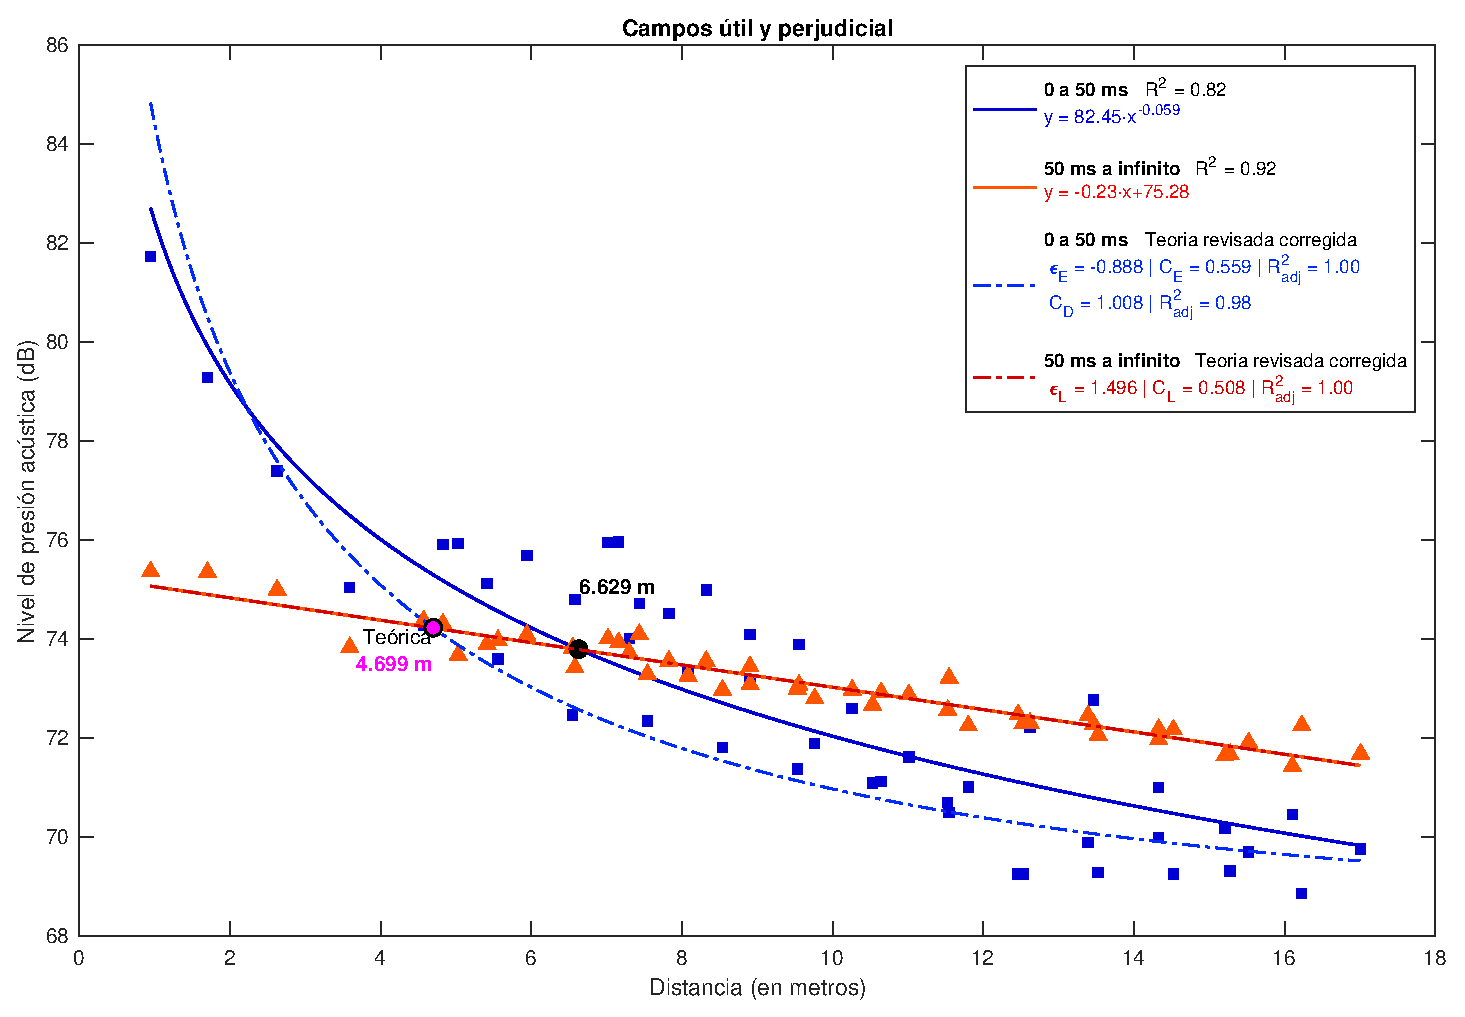
\includegraphics[width=0.8\textwidth]{archivos/capturas/dbfamatlab}
    \caption{Representación de curvas de medidas in situ y teóricas.}
\end{figure}
\FloatBarrier

La herramienta es compatible con los sistemas MacOS y Windows, y con versiones de Matlab desde 2014 y está disponible en la plataforma GitHub.














